This Chapter gives an overview of \acrlong{vo}, its working, different types of approaches and state-of-the-art of \acrlong{vo}.   

\section{Basics}
Localization of a robot is a fundamental challenge and one of the most
important tasks. For autonomous navigation, motion tracking, and obstacle detection and avoidance, a robot must know of its position in real time. Vision-based Odometry is a novel and robust solution utilized for this purpose.\cite{Aqel-et-al-2016} It allows a robot to localize itself accurately by using only a stream of images captured by a camera attached to the vehicle.

\begin{figure}[h]
	\centering
	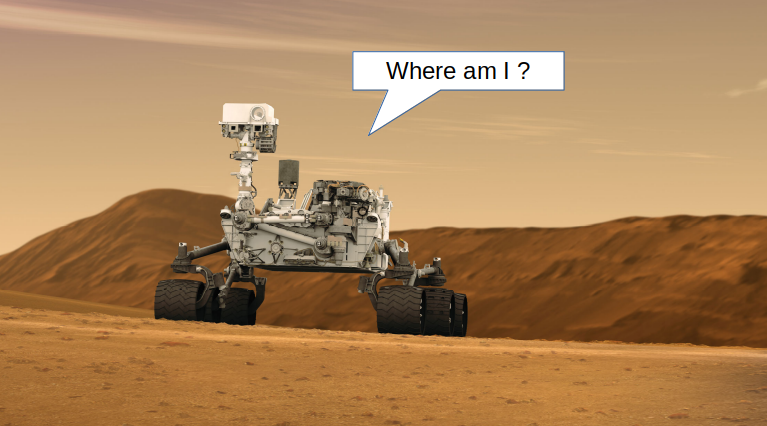
\includegraphics[width=0.5\textwidth]{where_am_i}
	\caption{NASA Path finder robot\cite{Online}]}
\end{figure}

\subsection{What is Visaul Odometry ?}
\acrshort{vo} is defined as the process of estimating the egomotion (translation and rotation with respect to a reference frame) of an Agent(e.g. vehicle, human and robot) by observing a sequence of images using single or multiple cameras attached to it.\cite{KhalidYousif-et-al-2015}] VO is a particular case of a technique known as \acrfull{sfm} in Computer Vision that tackles the problem of 3D reconstruction of environment and camera poses from set of images\cite{ScaramuzzaVO}. \acrshort{vo} mainly focuses on 3-D motion of the camera sequentially in real time (sequential \acrshort{sfm}).\acrshort{vo} mainly differs with \acrshort{slam} in terms of global mapping. \acrshort{vo} focuses on local consistency and incrementally estimate the path of camera/robot pose, and some local optimization whereas \acrshort{slam} performs both localization and global mapping.

\subsection{VO Pipeline}
The VO pipeline is summarized in Figure \ref{fig:flow}. For every new image I(or image pair for stereo case), the first two steps consist of detecting and matching 2-D features with those from the previous frames. 2-D features that are the reprojection of the same 3-D feature across different frames are called image correspondences. The feature detection consists of detecting features independently in all the images and then then feature matching will find the same features in sequence of images and then tracks them using a local search technique, such as correlation. The next step consists of computing the relative motion(translation and rotation) between the two consecutive time instants. There are three different approaches for motion estimation depending on the correspondences specified in 3-D or 2-D. Current camera pose is then computed by concatenation of the previous pose. Finally, an iterative local optimization known as \acrshort{ba} can be done over the last m frames to obtain a more accurate estimate of the local trajectory. Each steps are discussed further in next section.

\begin{figure}[h]
	\centering
	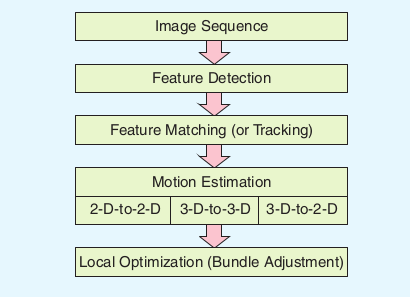
\includegraphics[width=0.5\textwidth]{vo_pipeline}
	\caption{Visual Odometry Pipeline}
	\label{fig:flow}
\end{figure}

\subsection{Types of VO}
\label{section:vo_types}

\acrshort{vo} mainly classified based on types of camera used for Such as stereo, monocular, omnidirectional, and RGB-D cameras (Fig.). Monocular \acrshort{vo} suffers from scale ambiguity because of unknown depth information of images. Stereo \acrshort{vo} solves this scaling problem by retrieving depth information using two cameras at little on distance known as baseline. Stereo case can be degraded to monocular if the baseline is much smaller than distances to the scene from the camera.\\
These methods are then further divided according to their approach as Indirect method(Feature based), Direct method(Intensity based) and Hybrid Approach (mixture of both approaches).

\subsubsection{Indirect Approach}

This is a classical approach for \acrshort{vo} and \acrshort{sfm}. The Indirect or Feature-based method involves extraction of some features such as corners, edges etc. from the images frames. See Figure\ref{fig:feature} These features are then matched and tracked among two consecutive image frames. Based on the feature tracking motion of camera is estimated.  This approach can typically divided into two steps: 1) Feature detection and matching, 2) geometric optimization on the computed point correspondences. In first step an image is matched with a previous one by comparing each feature in both images and calculating the Euclidean distance of feature vectors to find the candidate matching features.\cite{Aqel-et-al-2016} In second step using these match correspondences the camera motion and surrounding 3D geometry can be estimated. In case of stereo \acrshort{vo} the features are first compared with each image pair and thus depth information of feature can be estimated. In this approach the reprojection error is minimized using Bundle Adjustment because keypoints positions(geometric quantities) are used to compute camera pose. The Bundle adjustment problem is described as below. 

\begin{equation*}
	T_{k,k-1} = arg min_{T} \sum_{i} \| u^{'}_{i}- u_{i}\|^{2}_{\Sigma}
\end{equation*}
where   $u^{'}_{i} = \pi (P_{i},T_{k,k-1})$ , $ u_{i} $ is $ i^{th} $  pixel 2D positions and $ u^{'}_{i} $ is reprojected 2D pixel position using 3D projection $(\pi)$.  

\begin{figure}[h]
	\centering
	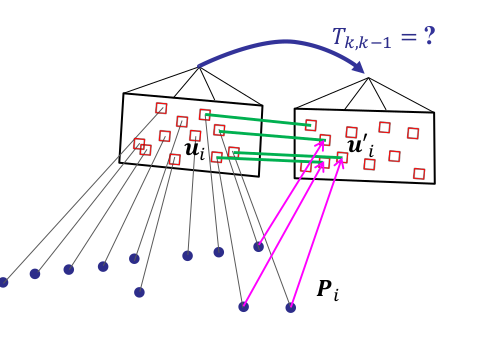
\includegraphics[width=0.5\textwidth]{indirect}
	\caption{Indirect method Optimizes Reprojection Error}
	\label{fig:feature}
\end{figure}

The disadvantage of feature-based approaches is their low speed due to feature extraction and matching at every frame, the necessity for robust estimation techniques that deal with erroneous correspondences (e.g., \acrshort{ransac} ), and the fact that most feature detectors are optimized for speed rather than precision.\cite{7782863}

\subsubsection{Direct Approach}

Direct method uses directly the pixel intensity as an information instead of extracting features and tracking them for motion estimation. Direct methods are based on assumption that Brightness remains constant in all image frames.\cite{Irani-et-al-1999} Direct methods are also known as Appearance based approach as it monitors the appearance of image in consecutive frames. The camera motion then can be estimated by Optical-flow algorithms which determines the displacement of brightness patterns of a group of pixels using intensity values from one image to another.\cite{Aqel-et-al-2016} There are two types of such algorithms based on selection of number of image pixels for calculation called as Dense and Sparse Optical-flow methods. Dense algorithms are less robust to noise as compared to Sparse based. Sparse algorithms select only those features which have more variance than others in particular image region. One of the most used sparse based algorithms for tracking is Lucas-Kanade method.\cite{Lucas81} As There is no feature extraction step is involved direct approach minimizes directly the photometric error formulated as below. 

\begin{equation*}
	T_{k,k-1} = arg min_{T} \sum_{i} \| I_{k}(u^{'}_{i})- I_{k-1}(u_{i})\|^{2}_{\sigma}
\end{equation*}

where   $u^{'}_{i} = \pi (P_{i},T_{k,k-1})$ and $I_{k} $ is  $k_{th}$ image. see Figure \ref{fig:direct}

\begin{figure}[h]
	\centering
	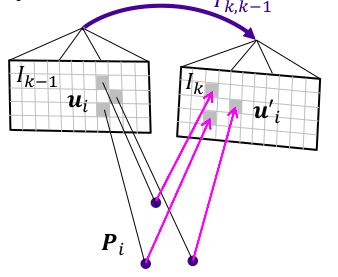
\includegraphics[width=0.5\textwidth]{direct}
	\caption{Direct Method Optimizes Photometric Error}
	\label{fig:direct}
\end{figure}

Depending upon the number of feature selection for calculating 3D geometry Direct methods can be divided into three types such as Dense, Semi-dense and Sparse methods.A graphical Overview of these methods can be seen in Figure \ref{fig:dense_sparse}. Dense approaches use every pixel in the image, where as semi-dense use just the pixels with high intensity gradient, and the proposed and sparse approach uses selected pixels at corners or along intensity gradient edges.\cite{engel14eccv}

\begin{figure}[h]
	\centering
	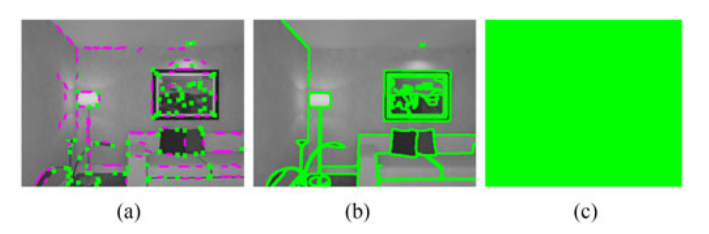
\includegraphics[scale=0.5]{dense_sparse}
	\caption{Image-to-model alignment (marked in green for corners and magenta for
		edgelets) for sparse, semi-dense, and dense methods. \cite{7782863} }
	\label{fig:dense_sparse}
\end{figure}

As Direct methods minimize the photometric error (intensity difference) for tracking between two images they required a well calibrated camera as compared to Indirect methods because they minimized the image pixel positions on images. A simple process comparison is described in the Figure.\ref{fig:direct_indirect}. Indirect methods have been very popular for a long time but recent advances in direct methods have shown better accuracy and robustness, especially when the images do not contain enough explicit corner features.\cite{Engel-et-al-pami2018} The robustness in the direct approach comes from the joint estimation of motion and correspondences as well as the ability to also use non-corner pixels, corresponding to edges, or even smooth image regions.\cite{gao2018ldso}

\begin{figure}[h]
	\centering
	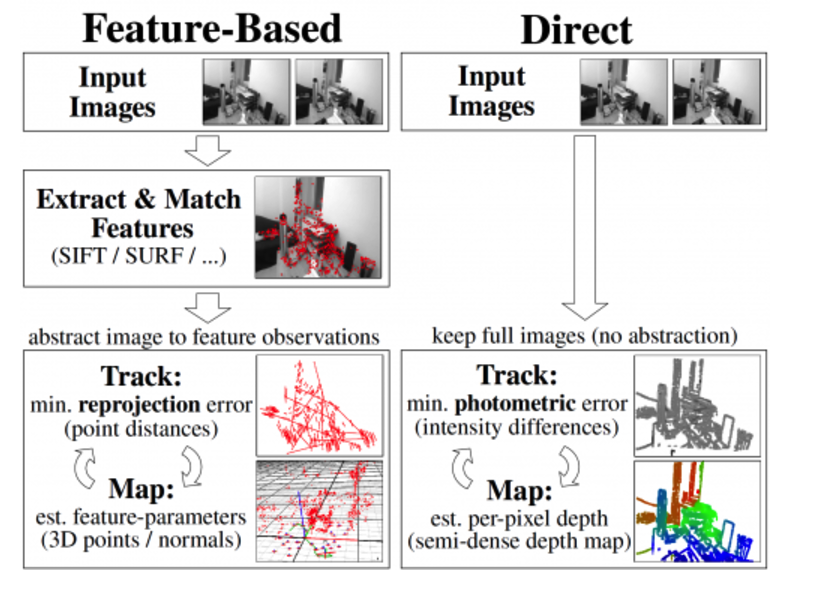
\includegraphics[width=0.5\textwidth]{direct_indirect}
	\caption{Process comparison between Direct and Indirect methods {source:\cite{engel14eccv}}}
	\label{fig:direct_indirect}
\end{figure}


\subsubsection{Hybrid Approach}
The indirect approach fails to deal with texture-less or low-textured environments of a single pattern such as sandy soil, asphalt, and concrete etc.. The less feature detection in these type of environments make this approach inefficient. While the direct approach is more robust and better than indirect approach in low-textured or single pattern environment but they are not much robust to image occlusions or inconsistencies in system (e.g rolling shutter). To have a advantages of both approaches the best solution is to use the combination of both approaches which combines tracking of salient features over over frames and use the pixel intensity as an information\cite{Aqel-et-al-2016}. Forster et al.\cite{7782863} proposed a hybrid approach in which they use a 4x4 patch around features and estimate the camera pose by minimizing the photometric error of these patches. For pose and structure refinement, the reprojection error of every feature is calculated with respect to the nearest keyframe that has observed the feature at nearly the same angle. \\

\subsubsection{Monocular vs Stereo}
In Monocular \acrshort{vo} a single camera is used for the whole pipeline. In this case features need to be observed in subsequent frames in order to track motion properly. Features observed in the first frame are triangulated into 3D points with help of second frame, and then transformation can be calculated using third frame \cite{KhalidYousif-et-al-2015}. While in stereo case, 3D points can be reconstructed (by triangulation) only by observing the features in the left and right images of a single pair simultaneously. Motion is estimated by observing features in two successive frames (both in left and right). Stereo approach has advantage of depth information of environment because it can obtain the disparity in scene. Where as monocular cameras can measure motion using pixel information only with no knowledge of scene depth. When the distance between scene to stereo camera becomes very long compared to the baseline(distance between left and right camera), the stereo case can be degraded to monocular because its very erroneous to measure the depth for far scene. 

\subsection{State of the Art}

\acrshort{vo} has been very active research topic in recent years. There has been many algorithms published based on the approaches discussed in section \ref{section:vo_types} and research is still ongoing. There are several papers which describes the current state of \acrshort{vo}. They are \cite{Aqel-et-al-2016}, \cite{KhalidYousif-et-al-2015} ,\cite{ScaramuzzaVO}. Currently research is focused based on the deep learning methods \cite{7989236} \cite{yang20d3vo} which is not in the scope of this thesis. Though \acrshort{vo} and \acrshort{v-slam} are widely researched topics it is still difficult to get an overview of all the algorithms. A list of various \acrshort{vo} and \acrshort{v-slam} algorithms, references and code if available can be found at \ref{section:A.1}. This list has been referred from \cite{chris}. The list presents mostly all algorithms invented so far. This thesis is based on the algorithms which work only based on camera. Also ,these algorithms can be classified according to their approaches. Considering these facts and other criteria such as \\
	1. runs on CPU  \\
	2. open source availability \\
	3. real-time \\
	4. state-of-the-art \\

three algorithms (one from each approach) \\
       1. \acrshort{orb}\acrshort{slam} \cite{Mur-Artal} \\
       2. Direct sparse odometry with loop closure (LDSO)\cite{gao2018ldso} \\
       3. Semi-direct visual odometry(SVO) \cite{7782863}  \\
       
are selected for implementation and later evaluation. In the next section these three algorithms their approaches, pros and cons compared to each other are described.  \\

\subsubsection{\acrshort{orb}\acrshort{slam}}

\acrshort{orb}\acrshort{slam} is a very popular feature(Indirect) based visual \acrshort{slam} approach. It uses an open-source \acrshort{orb} feature descriptors as feature extraction and matching, which was developed by Rublee et al.\cite{6126544}.These \acrshort{orb} features are robust to rotation and scale and also provides good invariance to auto-exposure and illumination changes. Further more they are fast to extract and match which makes them suitable for real-time applications\cite{Mur-Artal}. Mur-Artal et al. \cite{Mur-Artal} used an approach of parallel threads for \acrshort{orb}\acrshort{slam} similar to that of used in \acrshort{ptam} \cite{4538852}. It uses three main parallel threads:1) tracking 2) local mapping 3) loop closing. Loop closing is the thread of performing full \acrshort{ba}. A detailed approach is given in the figure \ref{fig:orbslam}.

\begin{figure}[h]
	\centering
	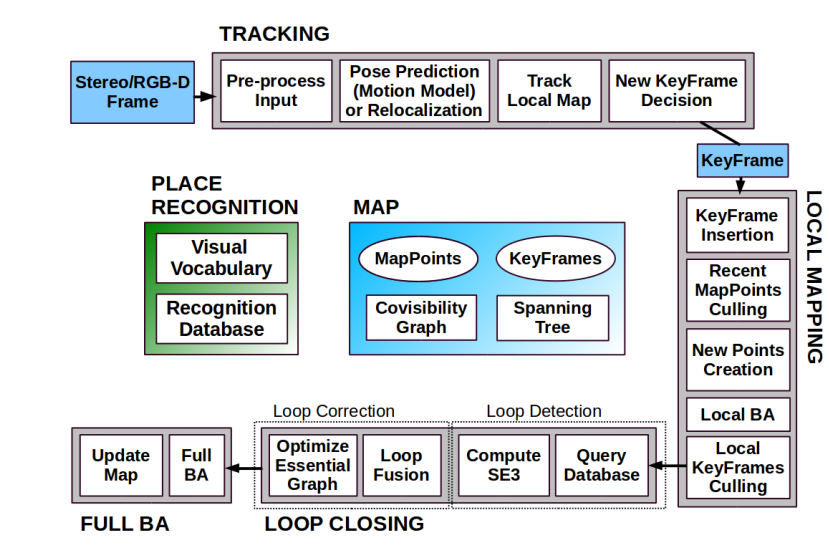
\includegraphics[width=0.5\textwidth]{orbslam}
	\caption{A process overview of \acrshort{orb}\acrshort{slam} \cite{Mur-Artal}}
	\label{fig:orbslam}
\end{figure}


\subsubsection{Direct Sparse Odometry}

\subsubsection{Semi-direct Visual Odometry}




